\documentclass[a4paper, 12pt]{article}
\usepackage{graphicx}
\usepackage{enumitem}
\usepackage{mathtools}
\def\code#1{\texttt{#1}}
\begin{document}

\title{\vspace{4.0cm}Applied GPU Programming - Assignment 1\\
\large DD2360 HT20}
\author{Pontus Asp}
\date{\today}
\maketitle
\thispagestyle{empty}
\pagenumbering{roman}
\newpage

\clearpage
\pagenumbering{arabic}

% Write here ->
\section{Exercise 1}
\begin{enumerate}
	% Why GPUs emerged as suitable hardware for computer graphics (e.g. games)?
	\item GPUs emerged as suitable hardware for computer graphics because computer graphics needs to calculate a lot of pixels. Most of the time the pixels can be independently calculated from each other and therefore are also susceptible to parallelization. The nature of GPUs are that they work great with calculating highly parallelized single instructions on multiple data (SIMD), like pixels in an image and make a perfect fit for this application.
	
	% Why do we talk about throughput-oriented architecture when we talk about GPUs?
	\item When talking about GPUs we talk about throughput-oriented architecture because that is the type of architecture that the GPUs use. It is thanks to this architecture that GPUs are highly efficient at handling SIMD operations.
	
	% List the main differences between GPUs and CPUs in terms of architecture.
	\item The main differences in the architecture between CPUs and GPUs are that the GPUs have many more computational units than a CPU. The GPUs architecture is made to maximize the amount (thoughput) of calculations per unit of time when the calculations are independent and has the same instructions but on different data. While the architecture of the CPU is better at handling instructions with less parallelization.
	
	% Use the Internet to find out and list the number of SMs, the number of cores per SM, the clock frequency, and the size of the memory of the NVIDIA GPU that you plan to use during the course. It might be the GPU of your laptop/workstation, or the GPUs on Tegner (Links to an external site.) (NVIDIA Quadro K420 or NVIDIA Tesla K80). Please, make sure that you mention the specific model as well.
	\item During this course I plan to use my own GPU, the NVIDIA GeForce GTX 1070. It has 15 SMs and 128 CUDA Cores per SM. The clock frequency is 1860 MHz and it has a memory of 8 GB. The specific name of the model is ROG-STRIX-GTX1070-O8G-GAMING.	
	
	% The new Nvidia GPUs (Volta, Turing, and Ampere) introduce two new kinds of cores, namely the Tensor and Ray Tracing cores.
	\item
	\begin{enumerate}[label=\arabic*.]
		% Which operation does the Tensor core support in one clock cycle?
		\item The Tensor core supports doing one multiply-and-accumulate on a 4x4 dimensional matrix per clock cycle.
		
		% What is the precision supported by Tensor cores?
		\item The Tensor Cores supports both taking input and matrix multiplication calculations in half floating-point precision but the accumulation uses single floating-point precision. How precise these precisions are, is decided in the IEEE 754 standard.
		
		% Why do you think that Tensor Cores were introduced in the new GPUs? For graphics or other applications?
		\item I think tensor cores were introduced in new GPUs mainly for the increasing demand of machine learning and their heavy use of matrix multiplication operations.
		
		% Check the Google TPU (also an accelerator) characteristic. What are the differences between GPUs with Tensor cores and TPUs?
		
		%%% (Section 4) Without sufficient operational intensity, a program is memory bandwidth-bound and lives under the slanted part of the roofline.
		
		%%% TPUs have better response-time (better at inference), while GPUs/CPUs typically have larger throughput, but does this apply to tensor cores?
		\item The biggest difference between the two other than the structure is response-time. TPUs have a better response-time while GPUs (also GPUs with Tensor cores) have better throughput.
		
		% Which operation does the Nvidia Ray Tracing core support in one clock cycle?
		
		%% The RT Core includes two specialized units. The first unit does bounding box tests, and the second unit does ray-triangle intersection tests.

		\item I have not been able to find any information on what operation the NVIDIA RT Core supports in a single clock cycle. However what I did find is that the NVIDIA RT Core accelerates calculating ray tracing. The RT Core has two specialized units, one which does bounding box tests and the other does ray-trinagle intersection tests.
	\end{enumerate}

	% Check the Top500 list (Links to an external site.) that is reporting the 500 most powerful supercomputers in the world. How many of the first 10 most powerful supercomputers use GPUs? Report the name of the supercomputers and the GPU vendor (Nvidia, AMD, ...) and model. 
	\item Six out of the ten most powerful supercomputers use GPUs, all of them use NVIDIA GPUs. The supercomputers names along with the GPU model is specified below.
	\begin{enumerate}[label=\arabic*.]
		\item Summit, NVIDIA Quadro GV100 Volta
		\item Sierra, NVIDIA Quadro GV100 Volta
		\item HPC5, NVIDIA Tesla V100
		\item Selene, NVIDIA A100
		\item Marconi-100, NVIDIA Tesla V100
		\item Piz Daint, NVIDIA Tesla P100
	\end{enumerate}
	
	%Use Google Scholar to find a scientific paper reporting about a work using GPUs in your main domain area (HPC, image processing, machine learning, ...). Report the title, authors, conference name/journal, the GPU type that has been used, and which programming approach has been employed.
	
	%%% SONG: Approximate Nearest Neighbor Search on GPU
	%%% Weijie Zhao, Shulong Tan, Ping Li
	%%% 2020 IEEE 36th International Conference on Data Engineering (ICDE)
	%%% NVIDIA TESLA V100
	%%% They approached their problem with using CUDA to perform graph based searches on ANNs using GPUs to speed up the searches.
	\item I found a paper related to machine learning.
	\newline \textbf{Title:} SONG: Approximate Nearest Neighbor Search on GPU
	\newline \textbf{Authors:} Weijie Zhao, Shulong Tan, Ping Li
	\newline \textbf{Converence:} 2020 IEEE 36th International Conference on Data Engineering (ICDE)
	\newline \textbf{GPU used:} NVIDIA TESLA V100
	\newline \textbf{Approach:} They approached their problem with using CUDA to perform graph based searches on ANNs using GPUs to speed up the searches.
\end{enumerate}
\newpage
\section{Exercise 2}
When running the bandwidthTest utility there was three (3) different tests, Host to Device Bandwidth (Figure \ref{fig:htd}), Device to Host Bandwidth (Figure \ref{fig:dth}) and Device to Device Bandwidth (Figure \ref{fig:dtd}) test.
My first observation was that the Device to Device test had a massively larger bandwidth than the other two tests. I realized this must be because the internal memory transfer rate is much higher than the transfer rate between the GPU and the rest of the system. My second observation was that the bandwidth in the transfer between the GPU and system seemed to have a roof at approximately 13 GB/s that it reached fast. I think it does not have the same speed when transferring very small amounts of bytes because of the latency in the transfer. Since the less bytes you transfer the bigger impact the latency has, which would explain the shape of the curve and why it flattens out so quickly. In Figure \ref{fig:dtd} there is a big drop in the bandwidth after $10^6$ in the X-axis. I am not sure why this happens but I would assume it has something to do with that since the transfer is between two locations in the GPU memory, the memory simply runs out while transferring when doing too big transfers so that it can not transfer with the same efficiency as before.
\begin{figure}
	\centering
	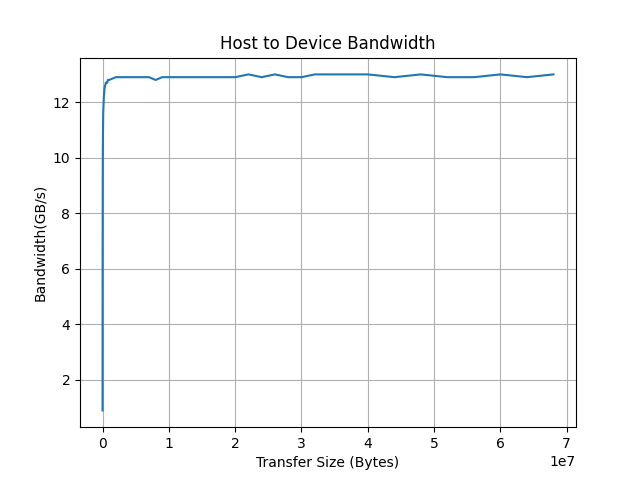
\includegraphics[width=0.8\linewidth]{host-to-device.png}
	\caption{Host to Device Bandwidth.}
	\label{fig:htd}
\end{figure}
\begin{figure}
	\centering
	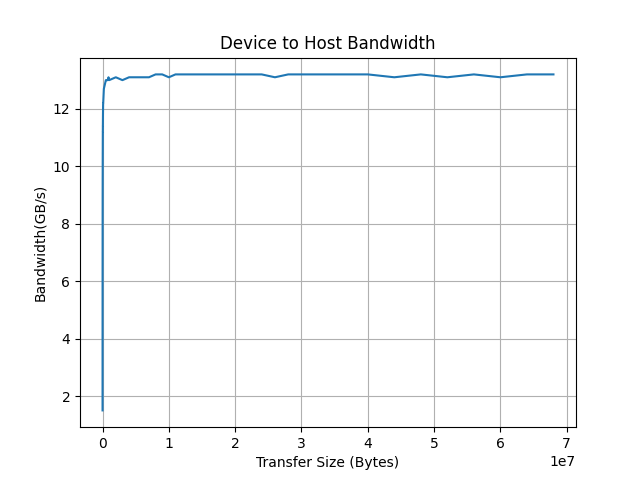
\includegraphics[width=0.8\linewidth]{device-to-host.png}
	\caption{Device to Host Bandwidth.}
	\label{fig:dth}
\end{figure}
\begin{figure}
	\centering
	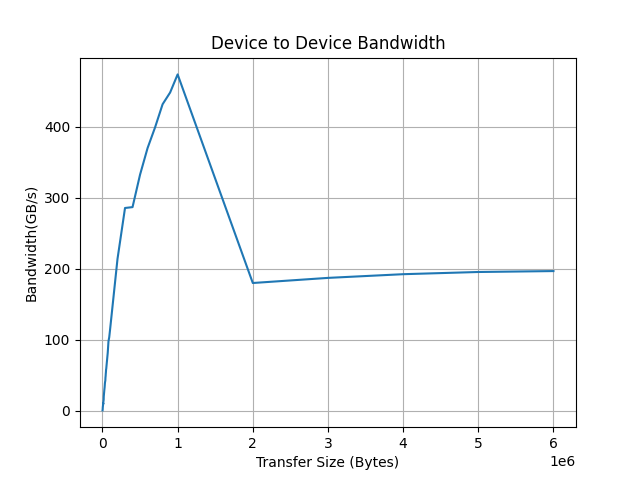
\includegraphics[width=0.8\linewidth]{device-to-device.png}
	\caption{Device to Device Bandwidth.}
	\label{fig:dtd}
\end{figure}
% Write here <--

\end{document}